


\chapter{Discrete Time System Implementation}

\section{Introduction}

The big question in this chapter is now how to build discrete time systems.\\

We know that the output of a system at an index $k$ is done via convolution, and there is 2 types of system: FIR and IIR.

\begin{equation}
\begin{array}{rcl}
y[\, k \,] \, &=& \, \displaystyle\sum\limits_{i \, = \, 0}^{k} h[\, i\,] \, x[ \, i \, - \, k \, ] \quad \text{IIR} \\ \\
y[ \, k \,] \, &=& \, \displaystyle\sum\limits_{i \, = \, 0}^{M \, - \, 1} h[\,i \,] \, x[\, i \, - \, k \, ] \quad \text{FIR} \\ \\
\end{array}
\end{equation}


\begin{itemize}

\item Notice that in IIR, the upper limit in $\displaystyle\sum $ is the same as the index of the output signal $y$

	\begin{itemize}
	\item This is a problem, because as $k$ increase, we need to add more terms via $h[i]$
	\end{itemize}

\item However in FIR, the upper limit is constant whatever the index $k$ we need to compute for.

	\begin{itemize}
	\item Each output needs $M$ multiplication and $M \, - \, 1$ additions
	\end{itemize}

\end{itemize}

\newpage
The FIR filter can be taught as the following block diagram:

\begin{figure}[h]
\centering
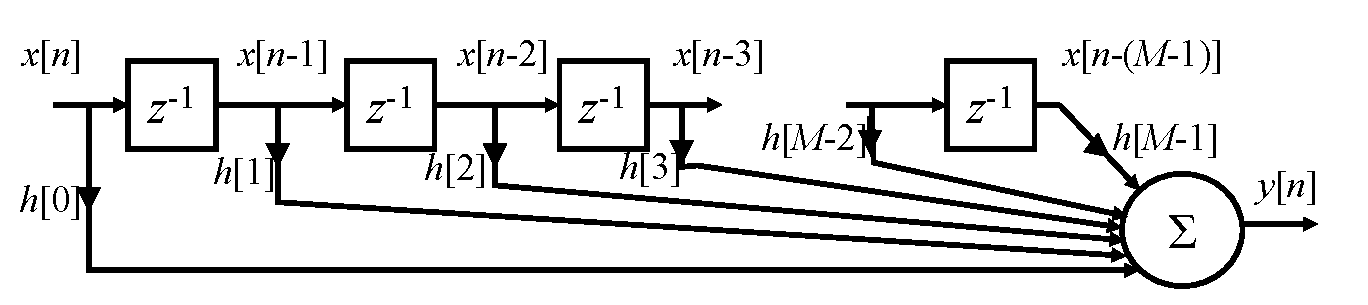
\includegraphics[width = 0.7\textwidth, frame]{Figures/discrete_time_systems/fir_block_diagram}
\caption{FIR Block Diagram}
\label{fig:discrete_time_systems:fir_block_diagram}
\end{figure} 


\begin{itemize}
\item We are assuming causal signal $x[n]$ and system $h[n]$

\item For each clock cycle, so for each value of index $n$:

	\begin{itemize}
	\item $y[0] \, = \, x[0] \, h[0]$, and all the other terms are 0 since we are causal system/signal
	
	\item In the next clock cycle $y[1]$: $x[0]$ gets shifted (the term $x[n \, - \, 1]$), and hence for $n \, = \, 1$ 
	
	
\begin{equation}
\begin{array}{rcl}
y[1] \, &=& \, x[n] \, h[0] \, + \, x[n \, - \, 1] \, + \, h[1] \\ \\
		 &=& x[1] \, h[0] \, + \, x[1 \, - \, 1] \,  h[1] \\ \\
		 &=& x[1] \, h[0] \, + \, x[0] \,  h[1] \, + \, \cdots
\end{array}
\end{equation}	
	
and all the other terms are 0

	\end{itemize}

\end{itemize}


The FIR block diagram shown in is called \tbi{feeforward} because everything is coming in forward direction to the $\displaystyle\sum$ block.


\section{IIR and Recursion}


Theoretically, convolution can implement FIR and IIR, but in IIR it poses problem regarding computation.\\

In this section, we see how we can implement \tbi{some} IIR system using recursion (feedback).\\

Consider the accumulator system:

\begin{equation}
y[n] \, = \, \displaystyle\sum\limits_{i \, = \, 0}^n x[i]
\label{Eq:discrete_time_systems:accumulator}
\end{equation}

which is an IIR system having an impulse response $h[n] \, = \, u[n]$. We can rewrite \autoref{Eq:discrete_time_systems:accumulator} as:

\begin{equation}
\begin{array}{rcl}
y[n] \, &=& \, \displaystyle\sum\limits_{i \, = \, 0}^n x[i] \\ \\		
		&=& \, \displaystyle\sum\limits_{i \, = \, 0}^{n \, - \, 1} x[i] + \, x[n] \\ \\
		&=& \, y[n \, - \, 1] \, + \, x[n]
\end{array}
\label{Eq:discrete_time_systems:accumulator_2}
\end{equation}

So to compute the current output sample $y[n]$, we need to save a value of the past output sample $ y[n \, - \, 1] $ and add the current input sample $x[n]$.\\

\autoref{Eq:discrete_time_systems:accumulator_2} lead to the concept of general $N^{\text{th}}$ order linear constant coefficient difference equation:

\begin{equation}
y[n] \, + \, a_1 \, y[n \, - \, 1] \, + \, \cdots \, + a_N \, y[n \, - \, N] \, = \, x[n] \, + \, b_1 \, x[n \, - \, 1] \, + \, \cdots \, + b_M \, y[n \, - \, M]
\label{Eq:discrete_time_systems:difference_eq}	
\end{equation}

\autoref{Eq:discrete_time_systems:difference_eq} can be rewritten in recursive form:

\begin{equation}
y[n] \, = \, - \, \displaystyle\sum\limits_{k \, = \, 1}^N a_k \, y[n \, - \, k] \, + \, \displaystyle\sum\limits_{k \, = \, 0}^M b_k \, x[n \, - \, k]
\label{Eq:discrete_time_systems:difference_eq_recursive} 
\end{equation}

\autoref{Eq:discrete_time_systems:difference_eq_recursive} can be used to compute the current output sample $y[n]$ using a finite amount of resources.


\section{Block Diagrams}

Block diagrams are the first step in implementing discrete time systems. They help us to define the internal structure of a discrete time systems, so they can help us when writing code or thinking about a specific hardware to implement and deploy discrete time systems.\\

We first begin from a specific example, and then take the results to generalize them.

\newpage
\subsection{First Order Difference Equation and Direct Form} 

Suppose we want to construct the block diagram of the following $\mathrm{1}^\mathrm{st}$ order difference equation:

\begin{equation}
y[n] \, = \, - \, a_1 \, y[n \, - \, 1] \, + \, b_0 \, x[n] \, + \, b_1 \, x[n \, - \, 1]
\label{Eq:discrete_time_systems:first_oder_difference_eq}
\end{equation}

\begin{itemize}

\item It is called $\mathrm{1}^\mathrm{st}$ order because the output samples $y[n]$ and $y[n \,  - \, 1]$ differ only by 1 sample

\item There are 2 delays: from input and output.

\end{itemize}

A straightforward block diagram of \autoref{Eq:discrete_time_systems:first_oder_difference_eq} is shown in 
\autoref{fig:discrete_time_systems:direct_form_1_first_order_diff_eq}.


\begin{figure}[h]
\centering
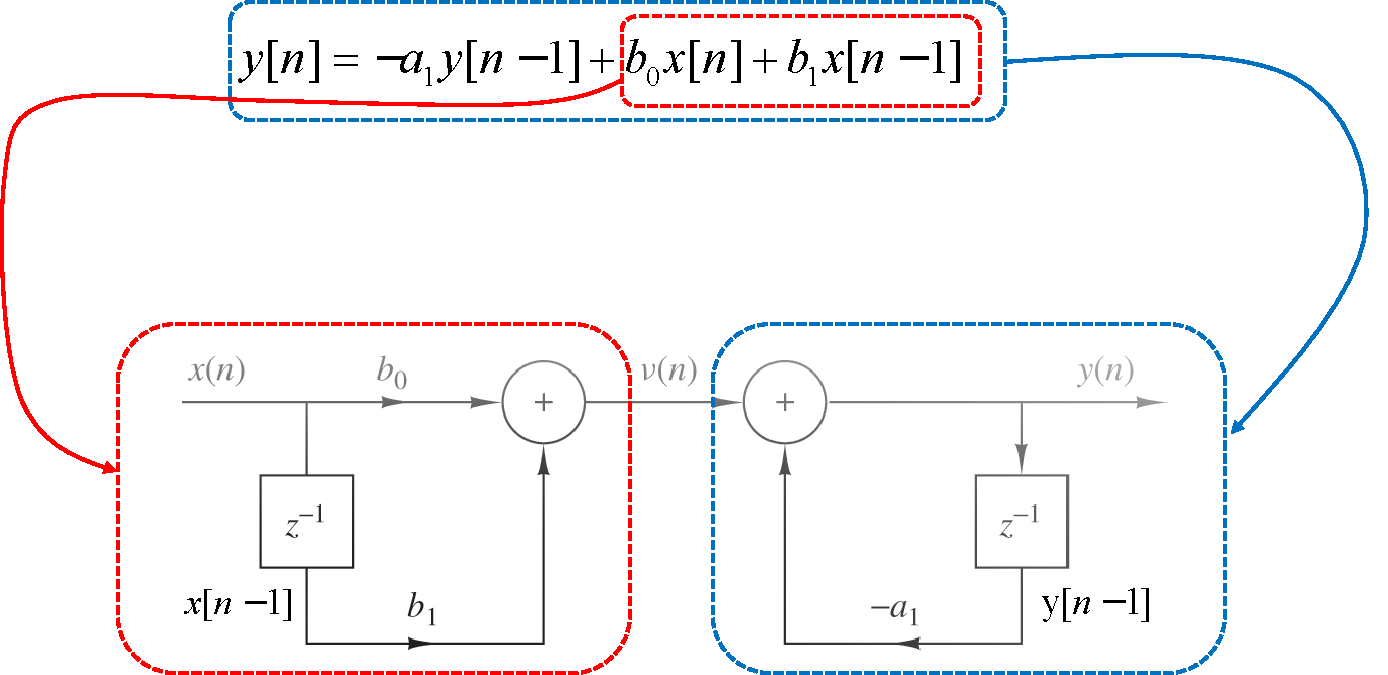
\includegraphics[width = 0.7\textwidth, frame]{Figures/discrete_time_systems/direct_form_1_first_order_diff_eq}
\caption{Direct Form I for $\mathrm{1}^\mathrm{st}$ order difference equation}
\label{fig:discrete_time_systems:direct_form_1_first_order_diff_eq}
\end{figure} 

\begin{itemize}

\item It is called \tbi{direct form I} because the delays of input and output are separated

\end{itemize}

Remember that delays elements are storage units (memory units) which holds previous samples, so the less we have memory the less resources we need.\\

\newpage
We can reduce delays elements by doing a handy trick: since we are working in LTI systems, we can \tbi{interchange the order of the systems without affecting the results}. Theses steps are shown in \autoref{fig:discrete_time_systems:interchange_order}.


\begin{figure}[h]
\centering
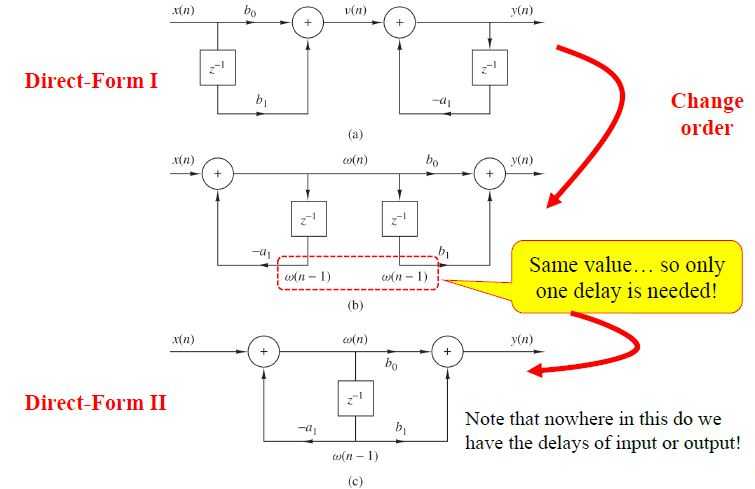
\includegraphics[width = 0.7\textwidth, frame]{Figures/discrete_time_systems/interchange_oder}
\caption{Interchanging order to reduce delay elements}
\label{fig:discrete_time_systems:interchange_order}
\end{figure} 

\begin{itemize}

\item Notice that in b), we have the same \tbi{intermediate number} $\omega(n)$ as input to the same delays, that's why we need 1 delay element only and not 2

\end{itemize}

Final results is shown in \autoref{fig:discrete_time_systems:direct_form_2_first_order}.

\begin{figure}[h]
\centering
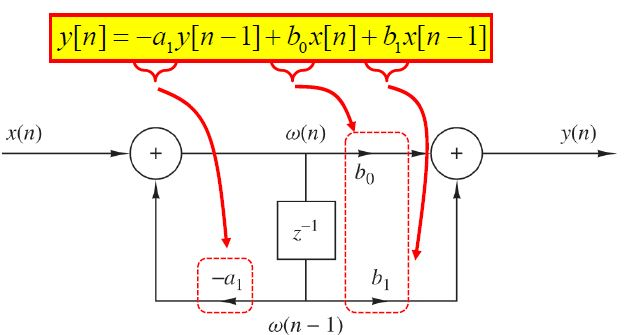
\includegraphics[width = 0.7\textwidth, frame]{Figures/discrete_time_systems/direct_form_2_first_order}
\caption{Direct form II for $\mathrm{1}^\mathrm{st}$ order difference equation}
\label{fig:discrete_time_systems:direct_form_2_first_order}
\end{figure}

\newpage
\subsection{General Direct Form}

Now we can generalize the direct form 1 and 2 from previous sections.


\begin{figure}[h]
\centering
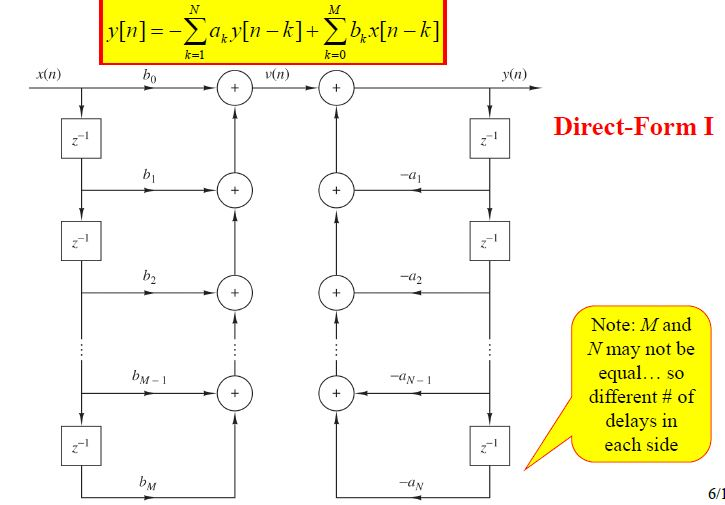
\includegraphics[width = 0.5\textwidth, frame]{Figures/discrete_time_systems/direct_form_1_general}
\caption{Direct form I General Form}
\label{fig:discrete_time_systems:direct_form_1_general}
\end{figure}

\begin{figure}[h]
\centering
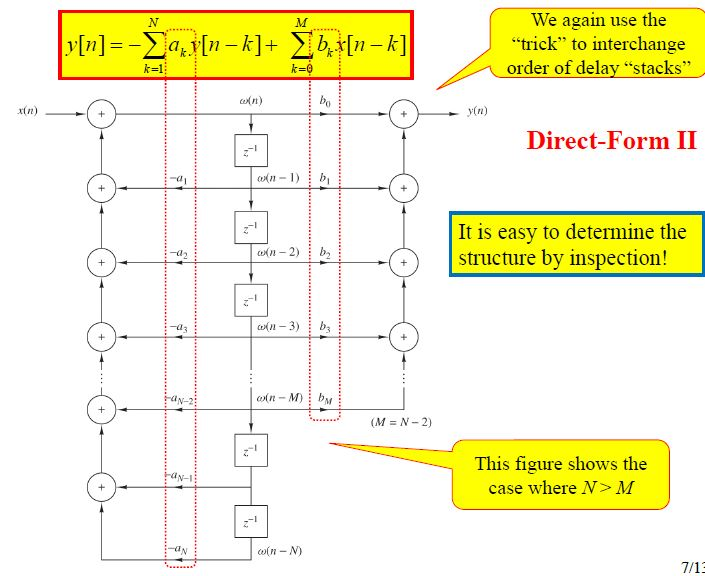
\includegraphics[width = 0.5\textwidth, frame]{Figures/discrete_time_systems/direct_form_2_general}
\caption{Direct form II General Form}
\label{fig:discrete_time_systems:direct_form_2_general}
\end{figure}

\begin{itemize}

\item Note that it is not necessary that $N \, = \, M$, so we can have different delay elements in direct form 1

\item For direct form 2: if $N \, \neq \, M$, we don't take branches always

\end{itemize}


\subsection{Recursion and Non Recursion}

Direct form 2 constitute from 2 parts: the $b_k$ (input coefficients), which are directly fed into the sum blocks, so they are \tbi{non-recursive}

\section{General Filter Design Concept}

Before diving into specific design technique for FIR or IIR, we present some general concept concerning filters in generals.

\begin{enumerate}

\item Discrete time filters present much more advantage over analog filters since we can use digital signal processing


\item Ideal response of a filter can't be achievable since the impulse response is a non-causal (sinc function)


\item We can only implement causal system

	\begin{itemize}
	\item Causal system are proven by Proney-Wiener Theorem, which give us a causal $h[n]$ for square integrable and convergent ln integral
	
		
		\item But also since we want the integral of the ln to converge, we can't allow for $H_{\text{filter}}(\omega_d)$ to take 0 on some interval, or the integral will blow up since ln 0 tends to $+\infty$, but we can have 0 values for some points $\leftrightarrow$ we can't have perfect stop band
				
	\end{itemize}


\item Structure of the Filter:

Proney-Wiener Theorem just says that mathematically we can obtain a causal response $h[n]$, but it doesn't state anything about the structure of the filter.\\

Our goal in filter design is to approximate some desired frequency response $H_{\text{desired}}$ using a rational transfer function.

	\begin{itemize}
	\item Why rational ? because using rational transfer function, we can implement filter using conventional block diagrams
	\end{itemize}

\item Practical Specifications: Every filter type have characteristics when designing: pass band, transition band, and ripples shown in 

\begin{figure}[h]
\centering
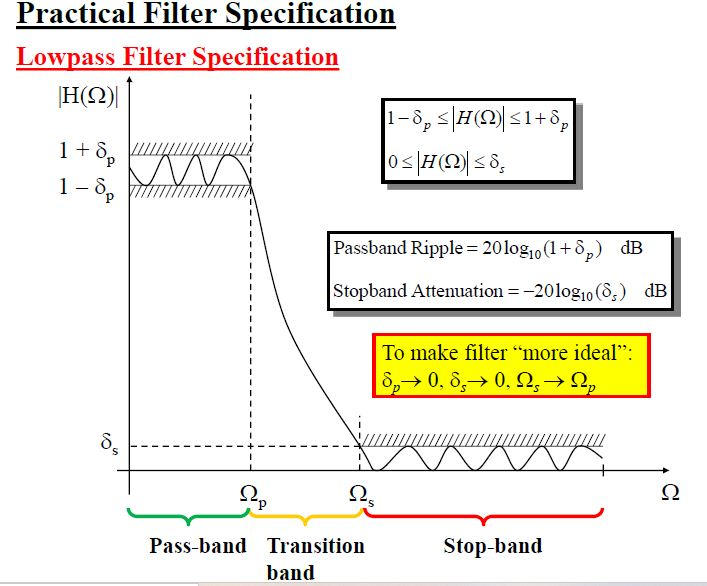
\includegraphics[width = 0.5\textwidth, frame]{Figures/discrete_time_systems/filter_specs}
\caption{Practical Filter Specification}
\label{fig:discrete_time_systems:filter_specs}
\end{figure}


	\begin{itemize}
	\item The more we approach ideal filter case $\leftrightarrow \, \delta_p \rightarrow \, 0 , \, \delta_s \rightarrow \, 0 $ and $\Omega_s \, \rightarrow \, \Omega_p$ (narrower transition band), the more the designing of the filter (IIR or FIR) become more complex
	
	
	\item Concerning the stop band attenuation: it is $ -20 \text{log}_10 \delta_s $, we put a - to make it positive because when we say attenuation, we say for example attenuation of 40 dB, but in reality it is -40 dB	
	
	\end{itemize}


\item FIR and IIR comparison: To do later.

	

\end{enumerate}